\section{Outras Estruturas}

\subsection{V-MOSFET}

\begin{frame}

    \begin{columns}[t]
    
        \begin{column}{7cm}

            \begin{itemize}
                \item Primeira estrutura;
                \item Dificil Fabricação;
                \item Instabilidade em uso prolongado;
                \item Ponta da porta prejudica a tensão de bloqueio
            \end{itemize}

        \end{column}

        \begin{column}{7cm}

            \begin{figure}[!htbp]
                \centering
                \caption{Estrutura V-MOSFET}
                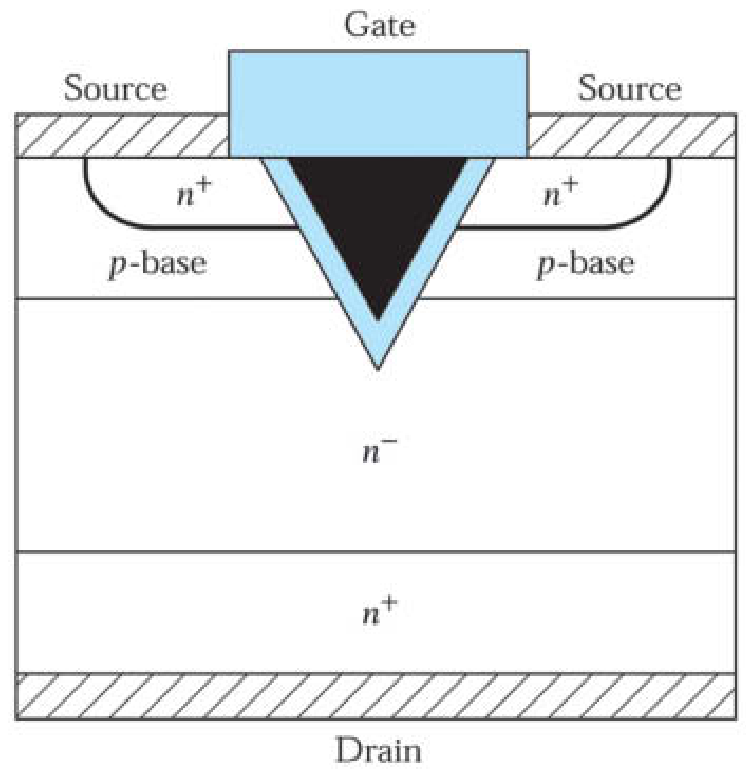
\includegraphics[scale=0.2]{imagens/vmosfet.png}
                \\\small{\textbf{Fonte:} \cite{sze2012semiconductor}}%
            \end{figure}

        \end{column}

    \end{columns}

\end{frame}


\subsection{U-MOSFET}

\begin{frame}

    \begin{columns}[t]
    
        \begin{column}{7cm}

            \begin{itemize}
                \item Estrutura mais nova;
                \item Menor R\textsubscript{on};
                \item Possibilitado por tecnologia usada em DRAM;
                \item Melhor desempenho em altas frequências
            \end{itemize}

        \end{column}

        \begin{column}{7cm}

            \begin{figure}[!htbp]
                \centering
                \caption{Estrutura U-MOSFET}
                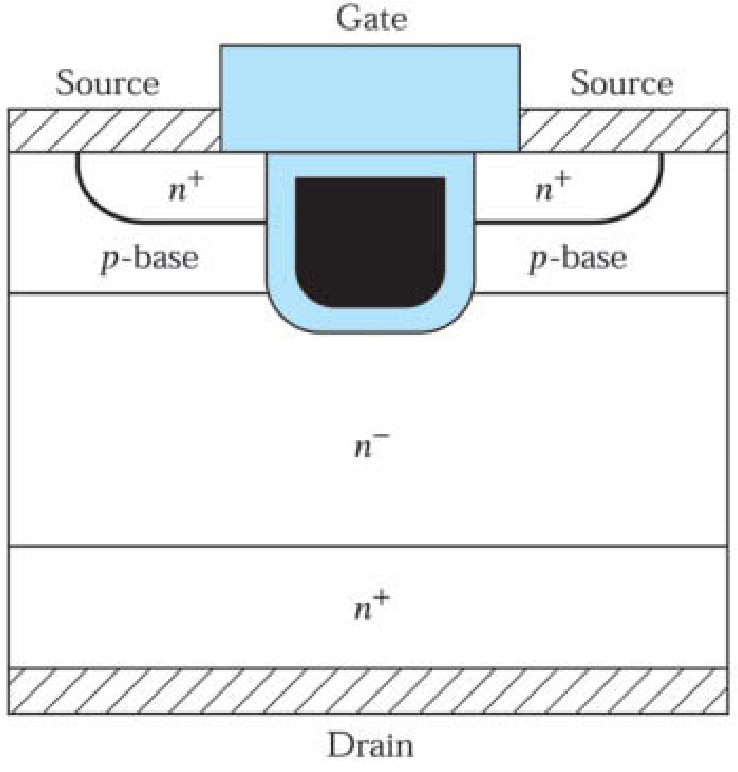
\includegraphics[scale=0.2]{imagens/umosfet.png}
                \\\small{\textbf{Fonte:} \cite{sze2012semiconductor}}%
            \end{figure}

        \end{column}

    \end{columns}

\end{frame}
